\q{On s’intéresse à la loi expérimentale de la somme de trois dés.}\\
\q{Construire une fonction }\il{Des_3(N)}\q{ qui donne expérimentalement la loi de la somme de trois dés
  lorsqu’on lance $N$ fois de suite trois dés ensemble. On pourra utiliser la fonction }\il{randint(a,b)}
\q{ de la bibliothèque }\il{random}\q{.}\\
\q{Pour $N = 8000$ lancers de trois dés, vérifier que la loi expérimentale présente une erreur d’environ 5\% par
  rapport au maximum de la loi théorique.}

\begin{dinglist}{111}
  \newpage
  \item
  Je crée d'abord la fonction \il{Des_3} :
  \codeFromFile{section-07/q7-1.py}

  \item
  Ensuite, pour \il{e} expériences, je fais \il{l} lancés, et j'enregistre les erreurs entre la loi théorique
  (\il{Th}) et la loi expérimentale (\il{Xp}). Ensuite je trace tout ça.
  \codeFromFile{section-07/q7-2.py}
  En exécutant \il{print(TraceExp(50, 8000) * 100)}, j'obtiens : $e_{max} = $ \il{4.823192239858807}\%.
  \begin{center}
    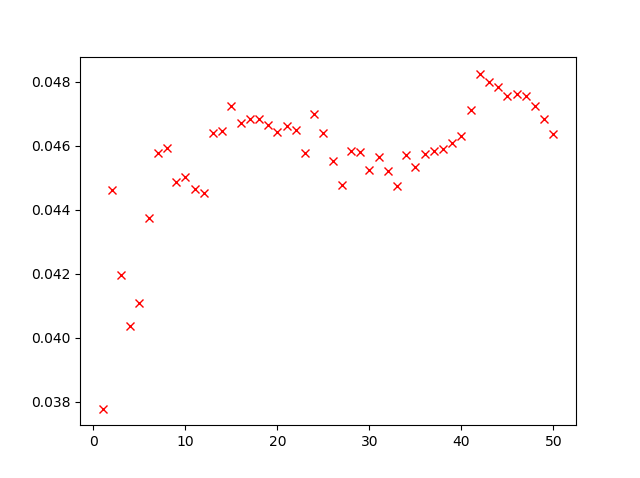
\includegraphics[scale=0.6]{section-07/q7-3.png}
  \end{center}
\end{dinglist}
